\documentclass[crop,tikz]{standalone}% 'crop' is the default for v1.0, before it was 'preview'
%\usetikzlibrary{...}% tikz package already loaded by 'tikz' option
\usepackage{color}
\newcommand{\gv}[1]{\ensuremath{\mbox{\boldmath$ #1 $}}} 
\renewcommand{\v}[1]{\ensuremath{\mathbf{#1}}}
\newcommand{\name}[1]{_{\text{#1}}}
\usepackage{siunitx}
\usepackage{amsmath}
\usetikzlibrary{shapes,arrows,shadings,backgrounds,calc}
\definecolor{brown}{rgb}{0.59, 0.29, 0.0}
\begin{document}
\fontfamily{cmss}
{  \begin{tikzpicture}
    %Lipid molecule

    \node[fill=white,label={[fill=white,rectangle,xshift=0.in,yshift=0%2.8in
        ]\textbf{CG-mapping}}](dppc) at (-0.25,-0.5) {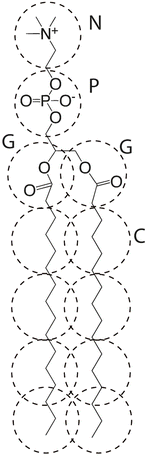
\includegraphics[height=2in]{DPPC_REP.png}};
    \node[circle,draw=black,dashed,label=left:{\scriptsize W}] (w) at ([yshift=-1.25in]dppc) {\scriptsize 4$\cdot$H$_2$O};
    %% \begin{pgfonlayer}{background}
    %%   \draw[ultra thick,opacity=1,blue] ([xshift=-1cm,yshift=-0.5cm]w.south west) rectangle ([xshift=0.25cm,yshift=0.25cm]dppc.north east); 
    %% \end{pgfonlayer}
      %Equations
    \node[fill=white,label=above:{\textbf{Intramolecular hamiltonian}}] (eq1) at (4,1.){
  $\begin{aligned}
     H_0=\sum&\frac {m_i\dot{\v r}_i^2}2  +\sum\frac {k_r(r_{ij}-r_0)^2}2+\\&\sum\frac {k_\theta(\cos(\theta_{ijk})-\cos(\theta_{0}))^2}2
  \end{aligned}$};%\( H_0=\sum\frac {m_i\dot{\v r}_i^2}2\v  +\sum\frac {k_r(r_{ij}-r_0)^2}2+\sum\frac {k_\theta(\cos(\theta_{ijk})-\cos(\theta_{0}))^2}2\)};

    %% \begin{pgfonlayer}{background}
    %%   \draw[ultra thick,opacity=1,blue] ([xshift=0cm,yshift=-0.5cm]eq1.south west) rectangle ([xshift=0.25cm,yshift=0.25cm]eq1.north east); 
    %% \end{pgfonlayer}

    % \node[](standard) at ([xshift=-0.75in,yshift=0.2in]eq1){\textbf{Intramolecular hamiltonian:}};
    
    %\node (eq2) at ([yshift=-0.5in]eq1){$\begin{aligned} W_0=\frac 1{2\rho_0}\int\text d \v r~(\sum_{k\ell}\textcolor{red}{\tilde\chi_{k\ell}}\phi_k(\v r)\phi_\ell(\v r)+\\ \frac{1}\kappa\left(\sum_\ell\phi_\ell(\v r)-a\right)^2)\end{aligned}$};
  
    
    %% %Kst
    \node[label=above:{\textbf{$W_1$-intercations}}](chi) at (4,-1.75){\scriptsize
      \begin{minipage}{1.7in}
        \begin{tabular}{cccc|r}
          \hline\hline
          G& P& C &W&\\
          \hline
          -1.50   &  6.30  &   9.00 &    -8.10&N\\
          & 4.50  &  13.50 &    -3.60&P\\
          &  &  6.30  &    4.50 &G\\                                                                                                                                 
          &  &   &    33.75&C\\
        \hline\hline
        \end{tabular}
      \end{minipage}
    };%label={[yshift=-2cm,xshift=-1cm]$\textcolor{red}{\tilde \chi_{k\ell$}} /\si{kJ.mol^{-1}}}
    \node (d) at ([xshift=1.1cm,yshift=.5cm]chi.south west){$\textcolor{red}{\tilde\chi_{k\ell}} /{\footnotesize \si{kJ.mol^{-1}}}$};
    %\draw ([yshift=0.25cm,xshift=0.3cm]chi.south)--([yshift=0.35cm,xshift=0.1cm]chi.west);
    
    \node[label=above:{\textbf{New modeling of tension}}] (eq3) at (4,-4){ \( W_1=-\frac 1{\rho_0}\int\text d \v r~\textcolor{blue}{K\name{ST}} \gv\nabla\phi\name{W}(\v r)\cdot\gv\nabla\phi\name{C}(\v r)\)};
     % \node(kst) at (4.5,-1.5){Water-carbon-interaction: $\textcolor{blue}{K\name{{ST}}}\equiv-K\name{{CW}}$};
    %% \node[anchor=west](kst1) at(3,-4.) {$\textcolor{blue}{K\name{ST}}<0$: \textit{Energy \textbf{loss} for surface area}};
    %% \node[anchor=west](kst1) at(3,-4.5){$\textcolor{blue}{K\name{ST}}>0$: \textit{Energy \textbf{gain} for surface area}};
  
  \end{tikzpicture}
}
\end{document}
